\documentclass[11pt,a4paper]{article}

% ---------- encoding & lingua ----------
\usepackage[utf8]{inputenc}
\usepackage[T1]{fontenc}
\usepackage[italian]{babel}
\usepackage{lmodern}

% ---------- layout ----------
\usepackage[a4paper,margin=2.4cm,headheight=14pt]{geometry}
\usepackage{microtype}
\usepackage{setspace}
\onehalfspacing
\usepackage{parskip}

% ---------- grafica ----------
\usepackage{graphicx}
\usepackage{xcolor}
\usepackage{tikz}
\usetikzlibrary{positioning,shapes.geometric,arrows.meta,calc,fit,backgrounds,decorations.pathreplacing}
\usepackage{booktabs}
\usepackage{array}
\usepackage{caption}
\captionsetup{font=small,labelfont=bf,width=0.95\textwidth}
\usepackage{enumitem}
\setlist{itemsep=2pt,topsep=3pt}
\usepackage{amsmath}
\usepackage{amssymb}

% ---------- intestazioni ----------
\usepackage{fancyhdr}
\pagestyle{fancy}
\fancyhf{}
\fancyhead[L]{\small\itshape Trentingrana Captioning}
\fancyhead[R]{\small\thepage}
\renewcommand{\headrulewidth}{0.4pt}

% ---------- titoli ----------
\usepackage{titlesec}
\titleformat{\section}{\Large\bfseries\color{prim}}{\thesection}{0.6em}{}
\titleformat{\subsection}{\large\bfseries\color{prim!85!black}}{\thesubsection}{0.6em}{}
\titlespacing*{\section}{0pt}{14pt}{6pt}

% ---------- colori ----------
\definecolor{prim}{HTML}{2C5F8A}
\definecolor{gold}{HTML}{E0A458}
\definecolor{green}{HTML}{5B8C5A}
\definecolor{red}{HTML}{C1492E}
\definecolor{m1c}{HTML}{E07A5F}
\definecolor{m3c}{HTML}{3D7068}
\definecolor{m6c}{HTML}{8A5082}
\definecolor{boxbg}{HTML}{F2F6FA}
\definecolor{boxbd}{HTML}{C7D6E5}

% ---------- link ----------
\usepackage[colorlinks=true,linkcolor=prim,citecolor=prim,urlcolor=prim]{hyperref}

% ---------- box riassuntivo ----------
\newcommand{\keybox}[2]{%
\begin{center}
\begin{tikzpicture}
\node[draw=boxbd,fill=boxbg,rounded corners=4pt,inner sep=8pt,
      text width=0.93\textwidth,align=left] {%
\textbf{\color{prim}#1}\\[2pt]\small #2};
\end{tikzpicture}
\end{center}}

% ============================================================
\begin{document}

% ---------------- FRONTESPIZIO ----------------
\begin{titlepage}
\centering
\vspace*{1.5cm}
{\color{prim}\rule{\textwidth}{2pt}}\\[0.6cm]
{\Huge\bfseries Captioning sensoriale del formaggio Trentingrana}\\[0.4cm]
{\LARGE Dalla costruzione del dataset al confronto di tre metodi encoder--decoder}\\[0.5cm]
{\color{prim}\rule{\textwidth}{2pt}}\\[1.2cm]

{\large Progetto \textbf{AI4FQC} --- Project 07: \textit{GRANA Captioning}}\\[0.3cm]
{\large Relazione tecnica esaustiva}\\[2.0cm]

\begin{tikzpicture}
\node[draw=boxbd,fill=boxbg,rounded corners=6pt,inner sep=14pt,text width=12cm,align=left]{
\setlength{\tabcolsep}{4pt}
\begin{tabular}{@{}l p{7.9cm}@{}}
\textbf{Dominio} & Analisi sensoriale di sezioni di forme di grana\\
\textbf{Acquisizione} & Analizzatore visivo elettronico IRIS\\
\textbf{Attributi} & 7 dimensioni sensoriali\\
\textbf{Dataset finale} & 38.437 coppie immagine--caption, 1.497 immagini\\
\textbf{Modelli} & m1 (CNN+LSTM), m3 (ViT+Transformer), m6 (ViT+GePpeTto)\\
\textbf{Costo LLM totale} & $\sim\$5{,}60$ (Anthropic Batch API, Haiku 4.5)\\
\end{tabular}};
\end{tikzpicture}

\vfill
{\large 2026}\\
\end{titlepage}

% ---------------- SOMMARIO ----------------
\section*{Sommario}
\addcontentsline{toc}{section}{Sommario}
Questa relazione documenta in modo completo il lavoro svolto nel progetto di
\emph{captioning sensoriale} del formaggio Trentingrana, articolato nei due
passi richiesti dalla traccia AI4FQC: (1) la pulizia e pre-elaborazione delle
descrizioni testuali dei degustatori, e (2) l'applicazione e il confronto di
tre metodi di captioning encoder--decoder concettualmente diversi.

Coerentemente con il peso effettivo del lavoro, circa il 70\% della relazione
\`e dedicato alla \textbf{costruzione del dataset} --- la parte pi\`u
complessa e originale del progetto --- e il restante 30\% alla
\textbf{selezione dei modelli e all'addestramento}. La pipeline di
preparazione dati trasforma 51.988 righe grezze, eterogenee e dialettali in
38.437 coppie immagine--caption pulite, normalizzate e in forma di frase
italiana, con un costo LLM contenuto a $\sim\$5{,}60$ grazie a una strategia
deterministica-prima-dell'LLM. Sul fronte modellistico, il risultato pi\`u
informativo emerge dallo \emph{shuffle test}: l'encoder visivo --- e non il
decoder --- \`e il fattore determinante per stabilire se il modello usi
davvero l'immagine.

\vspace{0.4cm}
{\small\tableofcontents}
\newpage

% ============================================================
\section{Introduzione e contesto}
% ============================================================

Il progetto nasce all'interno dell'iniziativa \textbf{AI4FQC}
(\textit{Artificial Intelligence for Food Quality Control}) e ha per oggetto
il \emph{Project 07 -- GRANA Captioning}. L'obiettivo \`e generare
automaticamente descrizioni sensoriali, in lingua italiana, a partire da
immagini di sezioni di forme di formaggio grana acquisite con l'analizzatore
visivo elettronico \textbf{IRIS} in condizioni di illuminazione controllata.

Ogni campione di formaggio \`e corredato da descrizioni redatte da un
\emph{panel} di degustatori esperti, che coprono \textbf{sette attributi
sensoriali}:
\begin{center}
\small
\begin{tabular}{@{}llll@{}}
\textcolor{prim}{$\blacksquare$} Profumo &
\textcolor{prim}{$\blacksquare$} Aroma &
\textcolor{prim}{$\blacksquare$} Sapore &
\textcolor{prim}{$\blacksquare$} Texture \\
\textcolor{prim}{$\blacksquare$} Spessore della Crosta &
\textcolor{prim}{$\blacksquare$} Struttura della Pasta &
\textcolor{prim}{$\blacksquare$} Colore della Pasta & \\
\end{tabular}
\end{center}

\subsection{I due passi della traccia}
La traccia richiede esplicitamente due deliverable:
\begin{enumerate}
\item \textbf{Passo 1 --- Pre-elaborazione del testo.} Pulire e normalizzare
le descrizioni telegrafiche, dialettali e incoerenti dei degustatori,
sostituendo in particolare le descrizioni quantitative (misure in mm/cm) con
descrizioni qualitative.
\item \textbf{Passo 2 --- Tre metodi di captioning.} Applicare e confrontare
tre metodi encoder--decoder ``concettualmente quanto pi\`u diversi
possibile''. L'enfasi \`e sul \emph{confronto di metodi}, non sulla ricerca di
un singolo modello ``migliore''.
\end{enumerate}

\subsection{Struttura della relazione}
La Parte~I (sezioni 2--11) ripercorre fase per fase la costruzione del
dataset, dalla tabella grezza al file finale, motivando ogni scelta tecnica.
La Parte~II (sezioni 12--16) descrive la scelta dei tre modelli, il setup di
addestramento su Kaggle, i risultati per-attributo e globali, e l'analisi di
\emph{image-conditioning}. Tutti i numeri riportati sono stati verificati
direttamente contro il codice e i file di dati del repository.

\keybox{In una riga}{2.745 fotografie + 13.159 commenti grezzi $\rightarrow$
pipeline di 11 fasi $\rightarrow$ 38.437 coppie immagine--caption pulite
$\rightarrow$ 3 metodi encoder--decoder confrontati su 7 attributi.}

% ============================================================
\part*{\centering\color{prim} Parte I --- Costruzione del dataset}
\addcontentsline{toc}{section}{Parte I --- Costruzione del dataset}
% ============================================================

\section{I dati grezzi e il problema del join}

Il punto di partenza era ingannevolmente ricco ma profondamente disallineato:
\begin{itemize}
\item \textbf{2.745 fotografie BMP} ($1024\times768$, RGB) di sezioni di forme,
organizzate per anno e per seduta. Ogni nome file codifica lo slot del panel,
l'identificativo del caseificio e la vista: \texttt{Fetta} (fetta della forma)
o \texttt{Grana} (primo piano della grana). Esempio:
\texttt{P3a\_TN306\_612\_Fetta.bmp}.
\item \textbf{Quattro workbook Excel} (uno per anno: 2018--2021), con un foglio
per attributo sensoriale. Ogni riga \`e il testo libero di un degustatore su
una forma per un attributo, pi\`u eventuali punteggi numerici.
\item \textbf{Un codebook} che mappa identificativi caseificio
$\leftrightarrow$ codici prodotto $\leftrightarrow$ lettere (16 caseifici).
\end{itemize}

\subsection{Il disallineamento centrale}
Il problema non ovvio era che \emph{immagini e commenti parlavano lingue
diverse}: i nomi file identificavano la singola forma (es. \texttt{612} \`e un
ID campione), mentre i commenti identificavano solo il \emph{vassoio} del
degustatore (\texttt{Prodotto = C0D}). Non esisteva un join a livello di riga:
solo un join a livello di \emph{caseificio}, attraverso il codebook.

\subsection{Decisione: broadcast a livello di caseificio}
Ogni commento del degustatore \`e stato propagato (\emph{broadcast}) a
\emph{tutte} le fotografie di quel caseificio in quella seduta. Un singolo
commento ``Crauti'' per il Profumo di un caseificio diventa cos\`i la caption
di pi\`u immagini (repliche \texttt{a}/\texttt{b} $\times$ viste
\texttt{Fetta}/\texttt{Grana}), fino a 4 righe immagine--caption da un solo
commento. La Figura~\ref{fig:broadcast} illustra il meccanismo.

\begin{figure}[t]
\centering
\begin{tikzpicture}[font=\small,
  cmt/.style={draw=red,fill=red!8,rounded corners=3pt,inner sep=6pt,text width=3.0cm,align=center},
  img/.style={draw=prim,fill=prim!8,rounded corners=3pt,inner sep=5pt,text width=2.3cm,align=center},
  arr/.style={-{Stealth[length=2.2mm]},prim,thick}]
\node[cmt] (c) {Commento panel\\\textit{``Crauti''}\\(Profumo, TN\_306)};
\node[img] (i1) at (5.2,2.1) {P3a -- Fetta};
\node[img] (i2) at (5.2,0.7) {P3a -- Grana};
\node[img] (i3) at (5.2,-0.7) {P3b -- Fetta};
\node[img] (i4) at (5.2,-2.1) {P3b -- Grana};
\foreach \i in {i1,i2,i3,i4} \draw[arr] (c.east) -- (\i.west);
\node[draw=green,fill=green!8,rounded corners=3pt,inner sep=6pt,
      text width=3.0cm,align=center] (out) at (10.4,0) {4 righe\\immagine--caption\\(stessa caption)};
\foreach \i in {i1,i2,i3,i4} \draw[arr] (\i.east) -- (out.west);
\end{tikzpicture}
\caption{Join per broadcast a livello di caseificio. In assenza di un join a
livello di forma, ogni commento \`e replicato su tutte le immagini coerenti.
Pi\`u righe per immagine sono un vantaggio per l'addestramento (pi\`u dati),
non un difetto.}
\label{fig:broadcast}
\end{figure}

L'effetto netto del join: \textbf{51.988 righe} (immagine $\times$ panelista
$\times$ attributo) su 2.745 immagini, di cui \textbf{39.510} con commento non
vuoto (tasso di pairing $\sim 76\%$, pi\`u basso nelle sedute 2021 dove alcuni
campi attributo erano lasciati vuoti).

\subsection{Anatomia di una difficolt\`a invisibile}
Tre ostacoli concreti, ognuno costato tempo reale, hanno reso il join non
banale:
\begin{itemize}
\item \textbf{Tripla indicizzazione del caseificio.} Lo stesso caseificio
appare nei dati come \texttt{TN\_306}, \texttt{TN306} e \texttt{306}; la mappa
di join li normalizza tutti alla stessa chiave per non perdere righe.
\item \textbf{Incoerenze di header tra anni.} ``Spessore della Crosta'' vs
``Spessore della crosta'', ``N\textordmasculine{} Seduta'' vs ``Seduta'':
normalizzati prima del merge.
\item \textbf{Virgola decimale italiana.} I punteggi numerici 2018
(\texttt{'7,48'}) richiedono parsing localizzato a \texttt{float}.
\end{itemize}
Tutti i metadati di provenienza (panelista, data seduta, caseificio, slot,
replica, vista) vengono propagati a valle, cos\`i ogni riga finale resta
tracciabile fino al commento originale.

\section{Architettura della pipeline}

La pipeline \`e organizzata in \textbf{11 fasi} (numerate 0--10), ognuna con un
proprio script Python, input/output espliciti e report ispezionabile. Il
principio guida \`e \emph{deterministico-prima-dell'LLM}: tutto ci\`o che pu\`o
essere fatto con codice riproducibile e gratuito viene fatto prima di
interpellare il modello linguistico. La Figura~\ref{fig:pipeline} ne mostra il
flusso complessivo.

\begin{figure}[t]
\centering
\begin{tikzpicture}[font=\footnotesize,node distance=3.0mm,
  ph/.style={draw=prim,fill=prim!8,rounded corners=3pt,inner sep=5pt,
             text width=3.2cm,align=center,minimum height=1.0cm},
  llm/.style={draw=gold,fill=gold!15,rounded corners=3pt,inner sep=5pt,
              text width=3.2cm,align=center,minimum height=1.0cm},
  fin/.style={draw=green,fill=green!12,rounded corners=3pt,inner sep=5pt,
              text width=3.2cm,align=center,minimum height=1.0cm},
  arr/.style={-{Stealth[length=2mm]},prim,thick}]
% colonna 1
\node[ph] (p0) {\textbf{0.} Tabella unificata\\\scriptsize 51.988 righe};
\node[ph,below=of p0] (p1) {\textbf{1.} Prep deterministica\\\scriptsize 39.356 righe};
\node[ph,below=of p1] (p2) {\textbf{2.} Vocabolario\\controllato};
\node[ph,below=of p2] (p3) {\textbf{3.} Audit vocabolario};
% colonna 2
\node[ph,right=2.0cm of p0] (p4) {\textbf{4.} Pulizia + qualitat.\\Spessore \scriptsize(7.705 uniche)};
\node[ph,below=of p4] (p5) {\textbf{5.} Drop rumore\\\scriptsize 7.689 al LLM};
\node[llm,below=of p5] (p6) {\textbf{6.} Design prompt\\\scriptsize 11 regole, 6 few-shot};
\node[llm,below=of p6] (p7) {\textbf{7.} Pilot run\\\scriptsize 105 caption};
% colonna 3
\node[llm,right=2.0cm of p4] (p8) {\textbf{8.} Batch completo\\\scriptsize 7.689 caption, Haiku 4.5};
\node[ph,below=of p8] (p9) {\textbf{9.} Salvage manuale\\\scriptsize +916 righe};
\node[fin,below=of p9] (p10){\textbf{10.} Broadcast + frase\\\scriptsize 38.437 righe};
\node[fin,below=of p10] (out){\textbf{Output}\\\scriptsize captions\_final.csv};
% archi
\draw[arr] (p0)--(p1); \draw[arr] (p1)--(p2); \draw[arr] (p2)--(p3);
\draw[arr] (p3.east)-- ++(0.4,0) |- (p4.west);
\draw[arr] (p4)--(p5); \draw[arr] (p5)--(p6); \draw[arr] (p6)--(p7);
\draw[arr] (p7.east)-- ++(0.4,0) |- (p8.west);
\draw[arr] (p8)--(p9); \draw[arr] (p9)--(p10); \draw[arr] (p10)--(out);
\end{tikzpicture}
\caption{Le 11 fasi della pipeline. In \textcolor{prim}{blu} le fasi
deterministiche (codice, gratuite), in \textcolor{gold}{oro} le fasi che
coinvolgono l'LLM, in \textcolor{green}{verde} l'assemblaggio finale.}
\label{fig:pipeline}
\end{figure}

La Figura~\ref{fig:funnel} quantifica come il numero di righe si riduce lungo
la pipeline a livello di \emph{broadcast} (righe di addestramento), mentre la
Figura~\ref{fig:funnelu} mostra la riduzione sul piano delle \emph{caption
uniche}, che \`e ci\`o che determina il costo dell'LLM.

\begin{figure}[h]
\centering
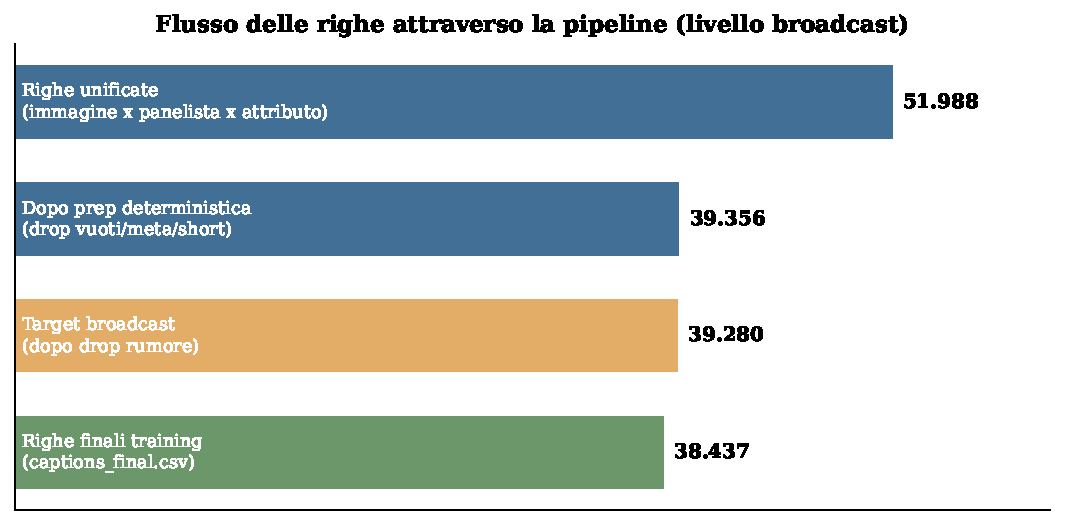
\includegraphics[width=0.92\textwidth]{figures/fig_funnel.pdf}
\caption{Flusso delle righe di addestramento attraverso la pipeline. Lo scarto
maggiore (12.632 righe) avviene nella prep deterministica, eliminando vuoti,
meta-commenti e frammenti senza contenuto.}
\label{fig:funnel}
\end{figure}

\begin{figure}[h]
\centering
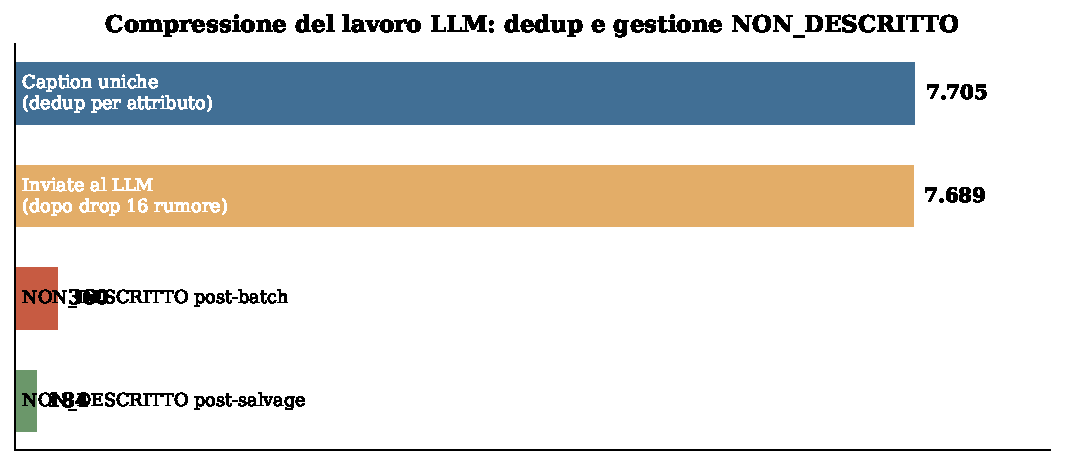
\includegraphics[width=0.92\textwidth]{figures/fig_funnel_unique.pdf}
\caption{Compressione del lavoro LLM. La deduplicazione riduce $\sim$39k righe
a 7.705 caption uniche (compressione $5{,}1\times$); solo queste vengono
inviate al modello.}
\label{fig:funnelu}
\end{figure}

\section{Fase 1 --- Preparazione deterministica}

La prima fase filtra e normalizza il testo \emph{senza riformularlo}. Le
operazioni principali:
\begin{itemize}
\item \textbf{Filtro righe vuote/N/A} e normalizzazione Unicode (NFC),
rimozione di spazi indivisibili (\texttt{\textbackslash xa0}), caratteri a
larghezza zero, tabulazioni e ritorni a capo.
\item \textbf{Drop di meta-commenti} via una piccola blacklist conservativa
(varianti di N/A, ``non penalizzo'', ``non valuto'', righe di sola
punteggiatura).
\item \textbf{Drop di rumore quasi-vuoto}: meno di 2 caratteri alfanumerici
dopo la pulizia.
\item \textbf{Doppia colonna} \texttt{caption\_raw} / \texttt{caption\_norm}
per garantire reversibilit\`a completa e auditabilit\`a.
\end{itemize}

L'output \`e di \textbf{39.356 righe} (75,7\% di retention), con
\textbf{12.632 drop} cos\`i ripartiti: 12.478 vuoti/null, 86 meta-commenti, 68
quasi-vuoti. Una scelta chiave \`e stata mantenere una blacklist
\emph{piccola}: a questo stadio i drop devono essere \emph{certi}, perch\'e
l'LLM gestir\`a meglio le ambiguit\`a (es. ``non penalizzo, ma sa di stalla''
contiene un descrittore reale e non va scartato).

\section{Fasi 2--3 --- Vocabolario controllato e audit}

Per ciascuno dei 7 attributi viene estratto un \textbf{vocabolario controllato}
dei lemmi e dei bigrammi pi\`u frequenti, con una lemmatizzazione italiana
\emph{custom} (mappe deterministiche di abbreviazioni e refusi, ripristino
degli accenti finali, dizionario \texttt{SPECIAL} per i casi ambigui, e un
merge corpus-driven singolare$\leftrightarrow$plurale che scatta solo quando
entrambe le forme sono attestate).

\subsection{Perch\'e un lemmatizzatore custom}
Le librerie NLP italiane standard sbagliano sistematicamente sul lessico
sensoriale (\texttt{panna}$\rightarrow$\texttt{panno},
\texttt{latte}$\rightarrow$\texttt{latto}). Inoltre includono nelle stopword
parole che qui \emph{sono} informative (\texttt{molto}, \texttt{poco},
\texttt{leggermente}, intensificatori sensoriali). Il vocabolario serve a due
scopi: (1) come base per l'audit, e (2) come \emph{ancora stilistica} nel
prompt LLM --- non come dizionario chiuso. Poich\'e il modello parla gi\`a
italiano fluentemente, non serve un lemmatizzatore perfetto: basta che la
forma canonica sia attestata.

La Figura~\ref{fig:vocab} mostra l'ampiezza del vocabolario per attributo.
\textit{Struttura della Pasta} \`e il pi\`u ricco (777 lemmi, 41.676 token),
\textit{Spessore della Crosta} il pi\`u povero (252 lemmi): coerente con la
loro diversit\`a descrittiva intrinseca.

\begin{figure}[h]
\centering
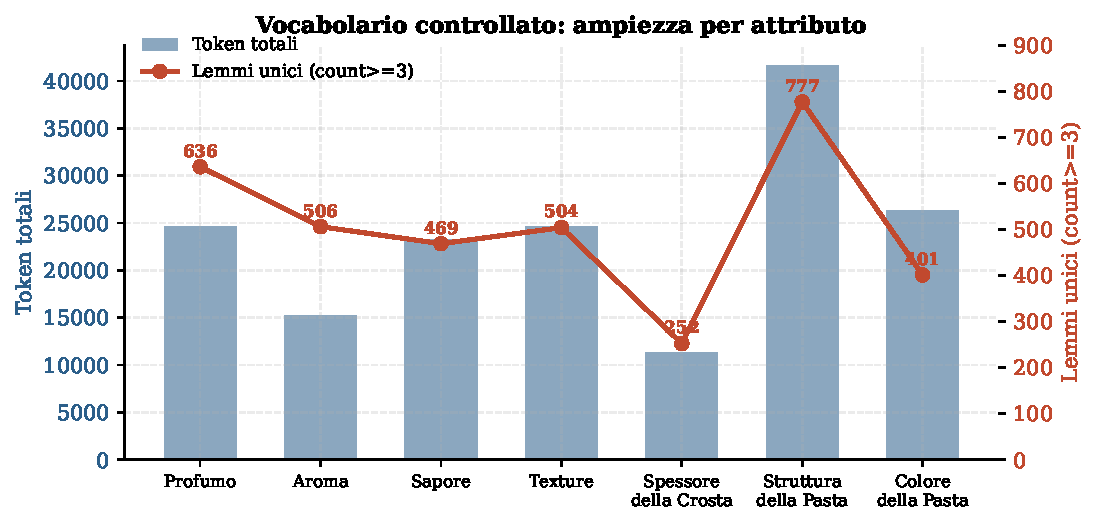
\includegraphics[width=0.9\textwidth]{figures/fig_vocab.pdf}
\caption{Vocabolario controllato per attributo: barre = token totali (asse
sinistro), linea = lemmi unici con frequenza $\geq 3$ (asse destro). La fase di
audit (\texttt{audit\_vocabulary.py}) ha segnalato token quantitativi, stem
spezzati e refusi tramite distanza di Levenshtein, in tre round di correzioni.}
\label{fig:vocab}
\end{figure}

\section{Fase 4 --- Pulizia e qualitatizzazione delle misure}

Questa fase deterministica esegue tre operazioni: pulizia testuale parola per
parola (espansione di abbreviazioni e refusi preservando il \emph{casing}),
\textbf{qualitatizzazione delle misure di crosta}, e \textbf{deduplicazione}.

\subsection{Da numeri a qualit\`a}
La traccia chiede esplicitamente di sostituire le descrizioni quantitative con
qualitative. Per lo Spessore della Crosta, centinaia di caption erano semplici
numeri (\texttt{10}, \texttt{1 cm}, \texttt{Mediamente 9 mm}, \texttt{8-10
mm}). Una funzione deterministica riconosce le caption \emph{interamente}
numeriche (con/senza unit\`a, range, prefissi-qualificatori), converte tutto in
millimetri (con euristica $<5 \rightarrow$ cm) e assegna un bucket
qualitativo:

\begin{center}\small
\begin{tabular}{@{}ll@{}}
\toprule
\textbf{Soglia (mm)} & \textbf{Bucket} \\
\midrule
$<8$ & Molto sottile \\
$8 \leq x < 10$ & Sottile \\
$10 \leq x < 14$ & Media \\
$14 \leq x < 18$ & Spessa \\
$\geq 18$ & Molto spessa \\
\bottomrule
\end{tabular}
\end{center}

Questo \textbf{elimina alla radice} la principale fonte di incoerenza
dell'LLM, che bucketizzava \texttt{1 cm} e \texttt{10 mm} (stessa misura
fisica) in modo diverso. La Figura~\ref{fig:spessore} mostra la distribuzione
risultante: 424 righe numeriche collassate in 5 bucket.

\begin{figure}[h]
\centering
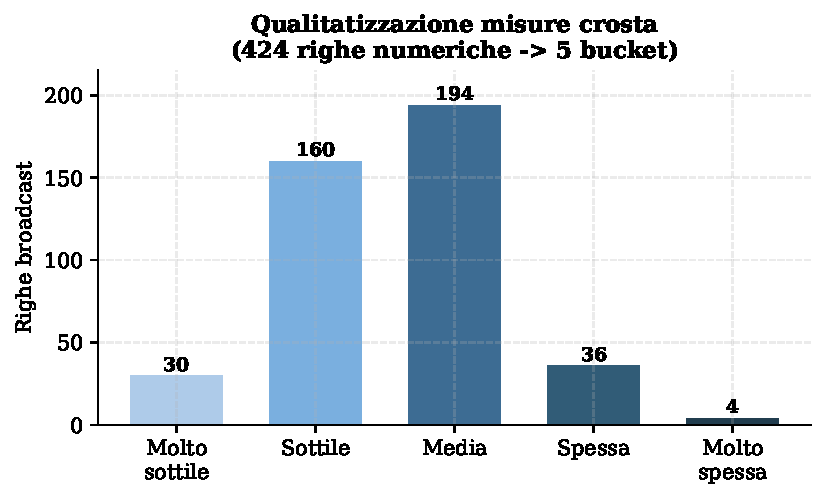
\includegraphics[width=0.6\textwidth]{figures/fig_spessore.pdf}
\caption{Qualitatizzazione delle misure di crosta. Le caption interamente
numeriche sono mappate deterministicamente sui 5 bucket; le caption miste
(es. ``spigoli sopra 20mm, piatto 10mm'') sono lasciate all'LLM perch\'e
richiedono ragionamento contestuale.}
\label{fig:spessore}
\end{figure}

\subsection{Deduplicazione}
A causa del broadcast, lo stesso testo sarebbe stato inviato all'LLM molte
volte. La deduplicazione per chiave \texttt{(caption, attributo)} comprime
39.356 righe in \textbf{7.705 caption uniche} (compressione $5{,}1\times$). La
Figura~\ref{fig:dedup} mostra la compressione per attributo. Questo \`e il
singolo accorgimento che riduce di $\sim 5\times$ il costo dell'LLM.

\begin{figure}[h]
\centering
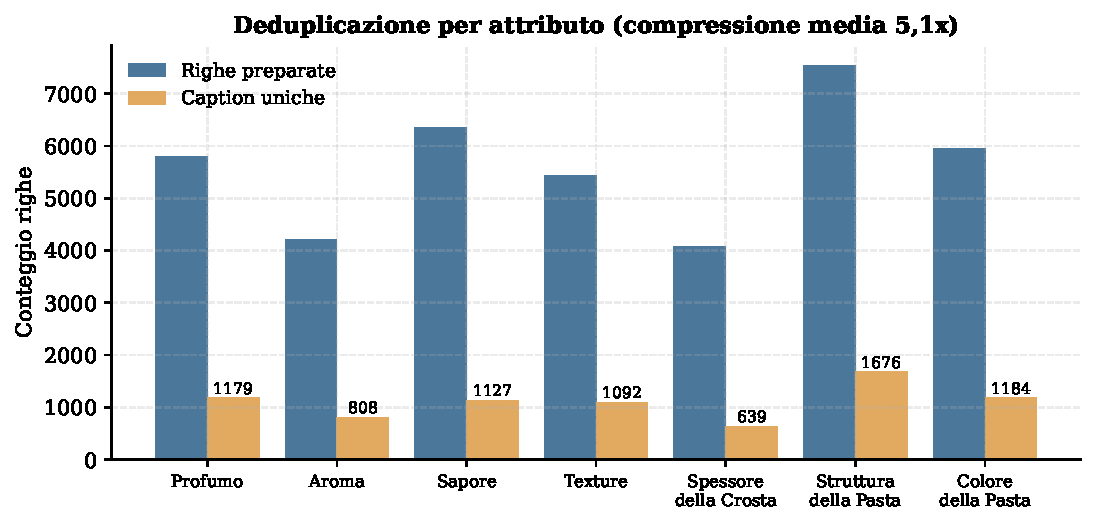
\includegraphics[width=0.9\textwidth]{figures/fig_dedup.pdf}
\caption{Righe preparate vs caption uniche per attributo. Il pattern dominante
di broadcast \`e $4\times$ (repliche \texttt{a}/\texttt{b} $\times$ viste
\texttt{Fetta}/\texttt{Grana}): 6.595 caption compaiono esattamente 4 volte.}
\label{fig:dedup}
\end{figure}

\section{Fase 5 --- Drop conservativo del rumore}

Uno script di \emph{survey} classifica le caption uniche in 7 categorie
(meta, valutazioni pure, intensificatori puri, incertezza, interrogativi, soli
numeri, vuoti post-tokenizzazione) senza droppare, producendo un report
ispezionabile. Solo successivamente uno script di \emph{drop attivo} elimina
le 3 categorie \emph{certe} (valutazioni pure come ``Buono''/``Ok'', soli
numeri fuori-Spessore, meta di sistema).

Il drop \`e deliberatamente conservativo: \textbf{16 caption uniche / 76 righe
broadcast (0,2\%)}. Le caption che mescolano meta e descrittore vengono
\emph{mantenute} --- l'LLM far\`a quella ``chirurgia'' meglio di una regex.
Vengono inoltre preservati gli interrogativi (``Eucalipto?'' $\rightarrow$ poi
trasformato in affermazione) e le negazioni descrittive (``Non paglierino''),
perch\'e portano informazione sensoriale reale. Restano \textbf{7.689 caption
uniche} pronte per il modello.

\section{Fasi 6--8 --- Riscrittura tramite LLM}

L'LLM svolge il lavoro genuinamente difficile che nessuna regex potrebbe fare
fedelmente: espandere parole telegrafiche in caption naturali (``Crauti''
$\rightarrow$ ``Profumo di crauti.''), normalizzare il dialetto, rimuovere i
meta-commenti preservando le parti descrittive, convertire misure
\emph{incorporate} in descrizioni qualitative e trasformare le domande in
affermazioni.

\subsection{Design del prompt (Fase 6)}
Un prompt di sistema per attributo ($\sim$5\,KB ciascuno) combina: ruolo e
framing del dataset, etichetta dell'attributo, template di stile,
\textbf{11 regole} (tra cui la regola 6 di ``zero invenzione'' e la regola 11
dell'escape \texttt{NON\_DESCRITTO}), regole extra per-attributo (tabella di
conversione mm/cm per lo Spessore), i \textbf{top-60 lemmi} del vocabolario
controllato come ancora stilistica, idiomi multi-parola curati a mano, e
\textbf{6 esempi few-shot} tratti da caption reali.

\subsection{Pilot run (Fase 7)}
Un campione stratificato di 105 caption (15 per attributo) \`e passato per
primo attraverso Haiku 4.5 in modalit\`a sincrona. Il pilot ha rivelato due
modi di fallimento, entrambi corretti nel prompt: (1) l'incoerenza
\texttt{1 cm} vs \texttt{10 mm}, risolta con la tabella di conversione
esplicita; (2) violazioni di formato sugli input senza contenuto, risolte con
l'escape \texttt{NON\_DESCRITTO}. Lezione operativa: 3 worker in parallelo
erano l'ottimo, 8 worker scatenavano tempeste di rate-limit (429).

\subsection{Batch completo (Fase 8)}
Tutte le 7.689 caption uniche sono state inviate come un singolo job Anthropic
Batch API: \textbf{7.689/7.689 completate, 0 errori}, $\sim$25--30 minuti,
$\sim\$4{,}50$. La Figura~\ref{fig:cost} motiva la scelta di Haiku 4.5: per
questo compito di riscrittura ben delimitato, verificato sul pilot, modelli
pi\`u costosi non offrivano alcun guadagno di qualit\`a misurabile.

\begin{figure}[h]
\centering
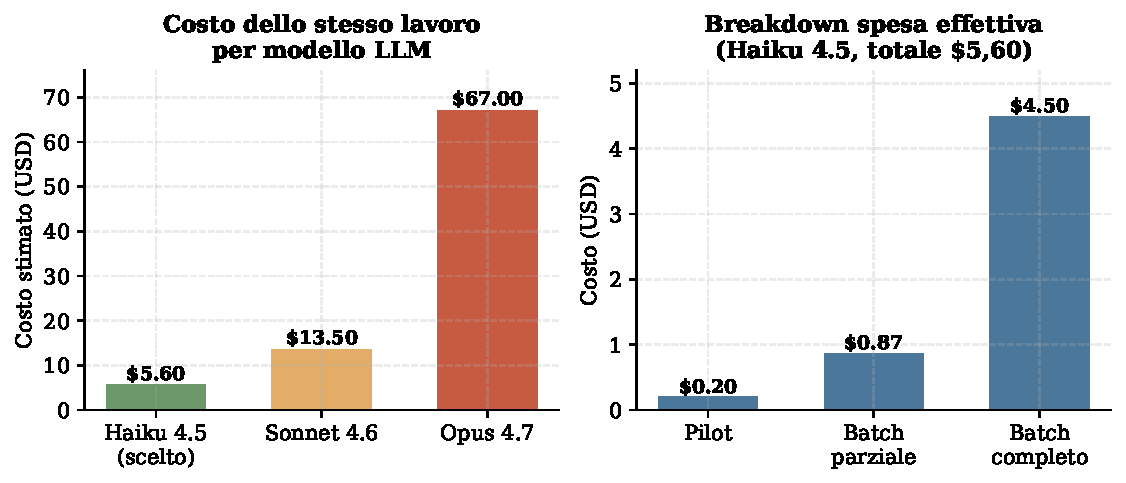
\includegraphics[width=0.92\textwidth]{figures/fig_cost.pdf}
\caption{A sinistra: costo dello stesso lavoro con modelli diversi --- Haiku
\`e $\sim$2,4$\times$ pi\`u economico di Sonnet e $\sim$12$\times$ di Opus. A
destra: ripartizione effettiva della spesa con Haiku 4.5 (totale $\$5{,}60$,
pilot + batch parziale + batch completo).}
\label{fig:cost}
\end{figure}

\subsection{Validazione programmatica dell'output}
Un controllo automatico su tutte le 7.689 uscite ha verificato la conformit\`a
al Passo 1 della traccia. Il risultato \`e netto:

\begin{center}\small
\begin{tabular}{@{}lc@{}}
\toprule
\textbf{Controllo} & \textbf{Violazioni} \\
\midrule
Output inizia col prefisso d'attributo atteso & 1 (prefisso alternativo valido) \\
Output contiene cifre & \textbf{0} \\
Output contiene unit\`a (mm/cm/\%) & \textbf{0} \\
Output pi\`u lungo di 25 parole & \textbf{0} \\
Output vuoto & \textbf{0} \\
Output multi-riga o con markup & \textbf{0} \\
\bottomrule
\end{tabular}
\end{center}

La conversione quantitativo$\rightarrow$qualitativo \`e riuscita al 100\%, una
soddisfazione pulita del requisito principale del Passo 1: \emph{zero numeri e
zero unit\`a di misura residue} nelle caption finali.

\section{Fase 9 --- Salvage manuale}

Una scansione euristica ha segnalato che 291 delle $\sim$362 caption taggate
\texttt{NON\_DESCRITTO} contenevano almeno un lemma del vocabolario
controllato --- segno che l'LLM era stato \emph{eccessivamente cauto} con la
regola 11 su input borderline (giudizio + descrittore). \`E stata curata a
mano una mappa di salvataggio di \textbf{178 caption} dove il descrittore era
reale e fedele:

\begin{center}\small
\begin{tabular}{@{}ll@{}}
\toprule
\textbf{Sorgente} & \textbf{Salvataggio} \\
\midrule
\texttt{"marcio, putrido,"} & ``Profumo marcio e putrido.'' \\
\texttt{"Strano. A tratti sentiva di pesce."} & ``Profumo strano, di pesce a tratti.'' \\
\texttt{"Sangue,,,"} & ``Aroma di sangue.'' \\
\texttt{"Anonimo"} & ``Aroma anonimo.'' \\
\bottomrule
\end{tabular}
\end{center}

L'effetto netto (Figura~\ref{fig:salvage}): i \texttt{NON\_DESCRITTO} unici
scendono da 362 a \textbf{184}, recuperando \textbf{916 righe di
addestramento}. Le caption rimaste \texttt{NON\_DESCRITTO} erano
genuinamente prive di informazione (giudizi puri, frammenti incomprensibili,
meta di sistema, osservazioni del tutto fuori-attributo).

\begin{figure}[h]
\centering
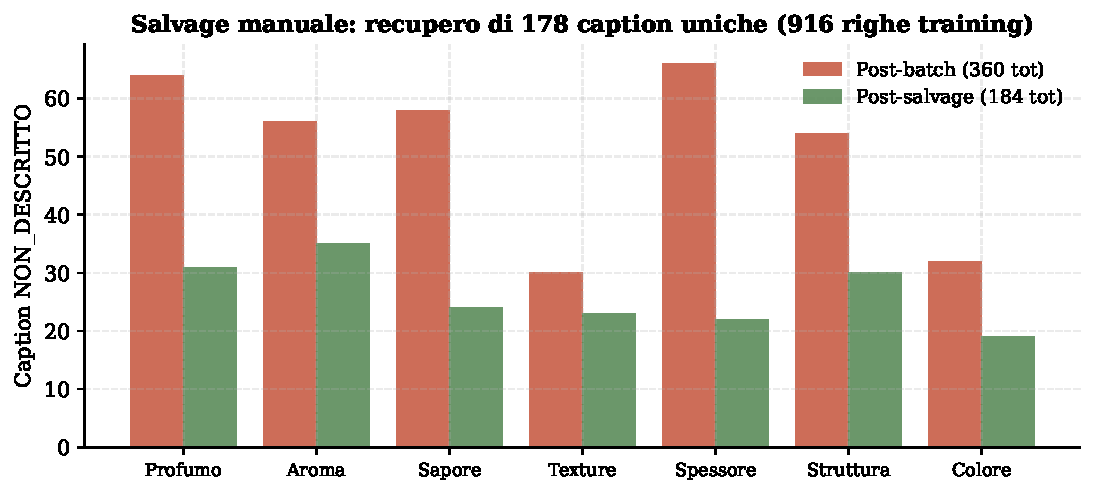
\includegraphics[width=0.9\textwidth]{figures/fig_salvage.pdf}
\caption{NON\_DESCRITTO per attributo, prima (post-batch, 360) e dopo
(post-salvage, 184) il salvataggio manuale. ``Pulire i dati'' non significa
``buttarli via'': la cura manuale ha recuperato 916 righe altrimenti perse.}
\label{fig:salvage}
\end{figure}

\section{Fase 10 --- Broadcast finale e forma di frase}

Le 7.505 caption pulite (escluse le \texttt{NON\_DESCRITTO}) vengono
riconnesse alla tabella broadcast di 39.280 righe tramite la chiave di
deduplicazione; le righe la cui caption pulita era \texttt{NON\_DESCRITTO}
vengono eliminate. Risultato: \textbf{38.437 righe} di addestramento su
\textbf{1.497 immagini uniche}.

\subsection{Forma di frase (sentence form)}
Un requisito tardivo: fornire, accanto alla forma compatta (\texttt{Profumo di
panna.}), una \textbf{frase italiana dichiarativa completa} (\texttt{Il
formaggio ha un profumo di panna.}), pi\`u adatta agli encoder--decoder e alle
metriche di captioning (BLEU, METEOR). La trasformazione \`e puramente
deterministica (nessun LLM): canonicalizzazione dei prefissi, sostituzione di
template, e un \emph{polish pass} che corregge le imperfezioni grammaticali
(iniezione dell'articolo dopo ``presenta'', consapevolezza dei plurali,
elisione \texttt{una}$\rightarrow$\texttt{un'}). Copertura template del 100\%,
zero round-trip LLM aggiuntivi.

Entrambe le forme sono presenti in ogni riga; \textbf{tutto l'addestramento
del Passo 2 usa la forma di frase} (\texttt{caption\_sentence}) perch\'e
grammaticale, pi\`u informativa e pi\`u rappresentativa di come un umano
descriverebbe il formaggio.

\section{Il dataset finale}

La Figura~\ref{fig:finalrows} riassume la distribuzione finale delle righe per
attributo. Vi \`e una varianza significativa (Struttura ha $\sim 1{,}9\times$
le righe di Spessore), fatto che incider\`a sul confronto cross-attributo nella
Parte~II.

\begin{figure}[h]
\centering
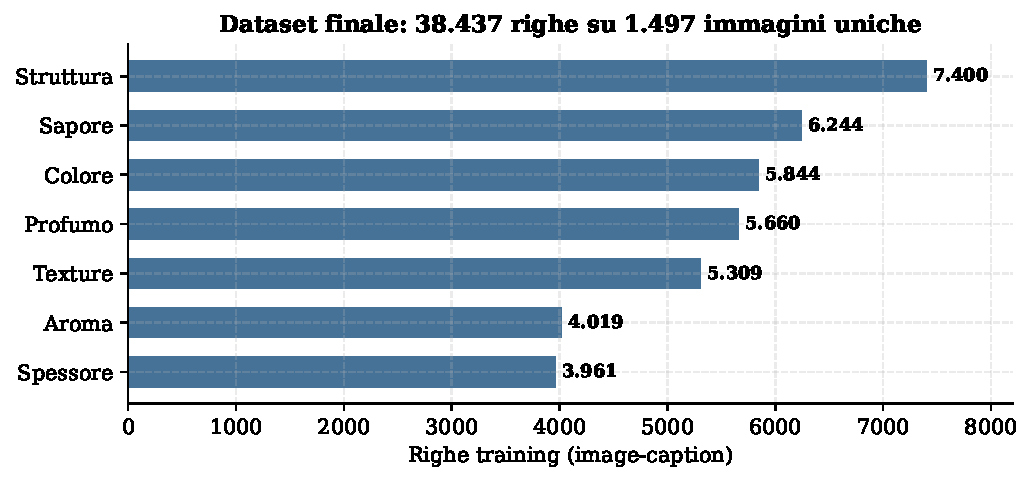
\includegraphics[width=0.86\textwidth]{figures/fig_final_rows.pdf}
\caption{Righe di addestramento per attributo nel dataset finale (38.437
totali). Ogni immagine contribuisce con una riga per attributo coperto.}
\label{fig:finalrows}
\end{figure}

\subsection{Schema del dataset consegnato}
Il deliverable del Passo~1 \`e fornito in pi\`u forme, per servire qualsiasi
architettura a valle:

\begin{center}\small
\begin{tabular}{@{}p{4.6cm} p{9.6cm}@{}}
\toprule
\textbf{File} & \textbf{Contenuto} \\
\midrule
\texttt{captions\_final.csv} & tabella completa, 38.437 righe $\times$ 18 colonne (provenienza inclusa) \\
\texttt{image\_caption\_attribute.csv} & vista semplificata a 4 colonne: \texttt{image\_path}, \texttt{attribute}, \texttt{caption}, \texttt{caption\_sentence} \\
\texttt{by\_attribute/<Attr>.csv} & 7 split per-attributo, per chi addestra un modello per attributo \\
\texttt{README.md} & spiegazione del deliverable per gli utenti a valle \\
\bottomrule
\end{tabular}
\end{center}

Ogni riga porta \textbf{due forme di caption}: \texttt{caption} (compatta,
$\sim$4--8 parole, ancorata all'attributo) e \texttt{caption\_sentence} (frase
italiana completa, $\sim$7--15 parole). Sono inoltre conservate tutte le
colonne di provenienza (panelista, data seduta, anno, vista, slot, replica,
caseificio, codice prodotto), cos\`i ogni coppia immagine--caption resta
tracciabile fino al commento originale del degustatore.

\subsection{Decisioni chiave e tradeoff}
La Tabella seguente raccoglie le scelte progettuali pi\`u rilevanti della
Parte~I, con la relativa motivazione --- la traccia chiede una pulizia ``in
modo accurato'', e ogni decisione \`e stata presa per essere auditabile e
giustificabile.

\begin{center}\small
\renewcommand{\arraystretch}{1.15}
\begin{tabular}{@{}p{3.2cm} p{5.0cm} p{4.7cm}@{}}
\toprule
\textbf{Decisione} & \textbf{Cosa} & \textbf{Perch\'e} \\
\midrule
Granularit\`a del join & Livello caseificio (broadcast a tutte le forme) & I dati non supportano un join a livello forma; pi\`u righe per immagine sono un vantaggio per il training \\
Deterministico prima dell'LLM & Pre-elaborazione pesante (typo, abbrev, qualitatizzazione, dedup) & Auditabile, gratuito, riduce il costo LLM di $\sim 5\times$ \\
Vocabolario come ancora & Top-N lemmi come ``preferisci'', non ``usa solo'' & L'LLM parla italiano; non serve un lemmatizzatore perfetto \\
Escape NON\_DESCRITTO & Token singolo invece di rifiuto multi-riga & Segnale banale da filtrare a posteriori \\
Salvage manuale & Cura a mano di 178 caption borderline & Recupera 916 righe; pi\`u economico di un altro giro LLM \\
Doppia forma caption & Compatta + frase nella stessa riga & A valle si sceglie quella adatta all'architettura \\
Haiku 4.5 (non Sonnet/Opus) & $\sim\$5{,}60$ vs $\sim\$13{,}50$ vs $\sim\$67$ & Il pilot ha provato che il modello piccolo gestisce il task con pari qualit\`a \\
\bottomrule
\end{tabular}
\end{center}

\keybox{Riepilogo Parte I}{Da 51.988 righe grezze e dialettali a 38.437 coppie
immagine--caption pulite, normalizzate e in forma di frase. Strategia chiave:
deterministico-prima-dell'LLM (dedup $5{,}1\times$, qualitatizzazione misure,
drop conservativo) per ridurre il costo LLM a $\$5{,}60$; salvataggio manuale
per recuperare 916 righe; doppia forma compatta/frase per la massima
flessibilit\`a a valle.}

% ============================================================
\part*{\centering\color{prim} Parte II --- Selezione dei modelli e training}
\addcontentsline{toc}{section}{Parte II --- Selezione dei modelli e training}
% ============================================================

\section{I tre metodi e gli assi di variazione}

La traccia chiede tre metodi encoder--decoder ``concettualmente quanto pi\`u
diversi possibile''. Sono state scelte tre architetture che isolano i tre assi
principali di variazione nel captioning di immagini (Figura~\ref{fig:arch}):

\begin{figure}[h]
\centering
\begin{tikzpicture}[font=\small,
  enc/.style={draw=prim,fill=prim!10,rounded corners=3pt,inner sep=5pt,text width=3.0cm,align=center,minimum height=1.1cm},
  dec/.style={draw=gold,fill=gold!15,rounded corners=3pt,inner sep=5pt,text width=3.0cm,align=center,minimum height=1.1cm},
  mod/.style={font=\bfseries\small},
  arr/.style={-{Stealth[length=2mm]},thick}]
% m1
\node[mod] (t1) at (0,3.4) {m1};
\node[enc] (e1) at (0,2.3) {ResNet-50\\\scriptsize (CNN, congelato)};
\node[dec] (d1) at (0,0.7) {LSTM\\\scriptsize da zero};
\draw[arr] (e1)--(d1);
% m3
\node[mod] (t3) at (4.2,3.4) {m3};
\node[enc] (e3) at (4.2,2.3) {ViT-B/16\\\scriptsize (congelato)};
\node[dec] (d3) at (4.2,0.7) {Transformer\\\scriptsize da zero};
\draw[arr] (e3)--(d3);
% m6
\node[mod] (t6) at (8.4,3.4) {m6};
\node[enc] (e6) at (8.4,2.3) {ViT-B/16\\\scriptsize (congelato)};
\node[dec] (d6) at (8.4,0.7) {GePpeTto\\\scriptsize GPT-2 italiano pre-addestrato};
\draw[arr] (e6)--(d6);
% assi
\draw[{Stealth[length=2mm]}-{Stealth[length=2mm]},red,thick] (e1.east)++(0,0) -- node[above,red,font=\scriptsize]{asse encoder} (e3.west);
\draw[{Stealth[length=2mm]}-{Stealth[length=2mm]},red,thick] (d3.east)++(0,0) -- node[above,red,font=\scriptsize]{asse decoder} (d6.west);
\end{tikzpicture}
\caption{I tre metodi e gli assi che isolano. \textbf{m1 vs m3} isola
l'\emph{encoder} (CNN vs ViT, stesso decoder da-zero); \textbf{m3 vs m6} isola
il \emph{decoder} (stesso ViT, decoder da-zero vs LM italiano pre-addestrato).
Tutti gli encoder sono \emph{congelati}: solo il decoder e la proiezione di
cross-attention vengono addestrati.}
\label{fig:arch}
\end{figure}

Tenere gli encoder congelati rende il confronto equo (stesse feature visive
disponibili a tutti i decoder) e mantiene il budget sperimentale gestibile. La
codebase implementa anche m2/m4/m5 per completare la griglia $2\times3$, ma non
sono stati eseguiti perch\'e non aggiungono un \emph{nuovo asse concettuale}.

\section{Setup sperimentale}

L'addestramento \`e avvenuto interamente sul tier GPU gratuito di
\textbf{Kaggle} (T4/P100). La Tabella seguente riassume gli iperparametri
(default ragionevoli per ciascuna architettura, non frutto di una ricerca):

\begin{center}\small
\begin{tabular}{@{}lccccc@{}}
\toprule
\textbf{Modello} & \textbf{epoche} & \textbf{batch} & \textbf{lr} & \textbf{scheduler} & \textbf{patience} \\
\midrule
m1 (CNN+LSTM) & 50 & 32 & $3\!\times\!10^{-4}$ & StepLR & 7 \\
m3 (ViT+Transf.) & 30 & 16 & $1\!\times\!10^{-4}$ & cosine & 5 \\
m6 (ViT+GePpeTto) & 20 & 8 & $5\!\times\!10^{-5}$ & cosine & 5 \\
\bottomrule
\end{tabular}
\end{center}

Lo split \`e \emph{sample-disjoint} (train 674 / val 143 / test 147 campioni):
lo stesso formaggio non compare mai sia in train sia in test, evitando il leak.
In inferenza, tutti i modelli decodificano con \textbf{nucleus sampling}
($\text{top-}p=0{,}9$, $T=0{,}7$) invece di beam search: su dataset piccoli il
beam collassa sulla caption modale, gonfiando il BLEU ma riducendo la
diversit\`a. Lezione Kaggle costosa: il flag \texttt{enable\_gpu} nei metadati
\emph{non} abilita davvero la GPU (va attivata manualmente), e il tier gratuito
tende a P100 (sm\_60) la cui PyTorch preinstallata va reinstallata da wheel
cu118.

\subsection{Salute dell'addestramento}
Prima dei risultati, vale la pena notare che le curve di addestramento sono
sane su tutti e tre i modelli: nessun segnale di overfitting, nessun
\texttt{NaN}, nessun collasso. m1 ha completato 50/50 epoche con
\texttt{val\_loss} in calo costante ($1{,}84 \rightarrow 1{,}04$); m3 si \`e
fermato in early-stop all'epoca 16/30 (patience 5); m6 ha completato 20/20 con
miglior \texttt{val\_loss} $1{,}06$ all'epoca 16. Le differenze nei risultati a
valle non sono quindi attribuibili a patologie di training.

\section{Risultati: per-attributo e globale}

I modelli sono stati valutati in due regimi: \textbf{per-attributo} (7 modelli
separati) e \textbf{globale} (un modello su tutti gli attributi insieme). La
Figura~\ref{fig:bleuattr} mostra il BLEU-4 per-attributo confrontato con la
baseline \texttt{most\_frequent} (che emette sempre la caption modale).

\begin{figure}[h]
\centering
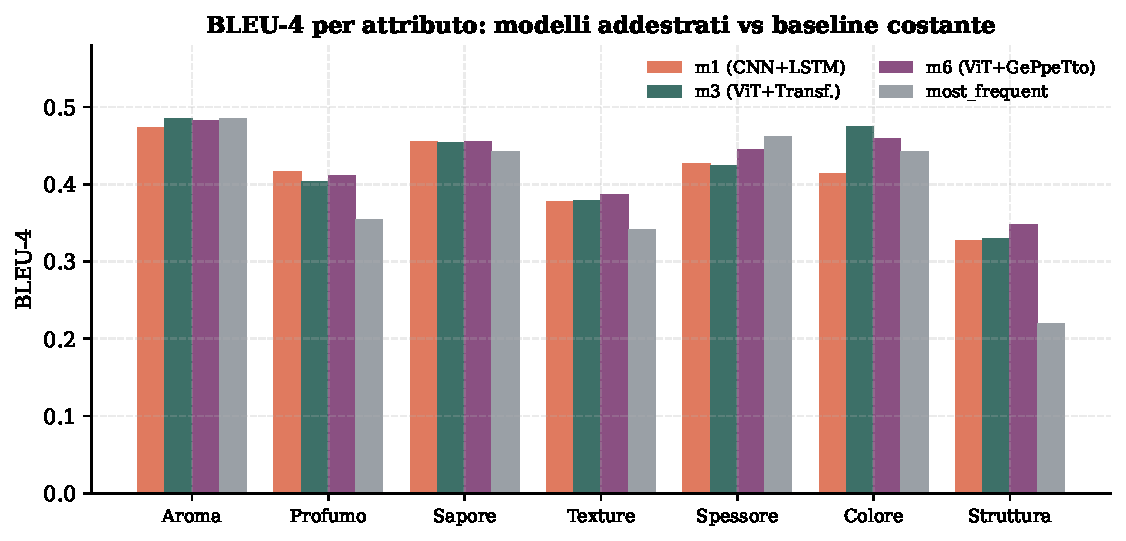
\includegraphics[width=0.95\textwidth]{figures/fig_bleu_attr.pdf}
\caption{BLEU-4 per attributo. I modelli addestrati battono nettamente la
baseline costante su Struttura ($+0{,}128$), Profumo, Texture e Colore; su
Aroma, Sapore e Spessore pareggiano o perdono --- non perch\'e siano scarsi,
ma perch\'e BLEU premia il predittore modale su distribuzioni di caption a
bassa diversit\`a.}
\label{fig:bleuattr}
\end{figure}

\begin{figure}[h]
\centering
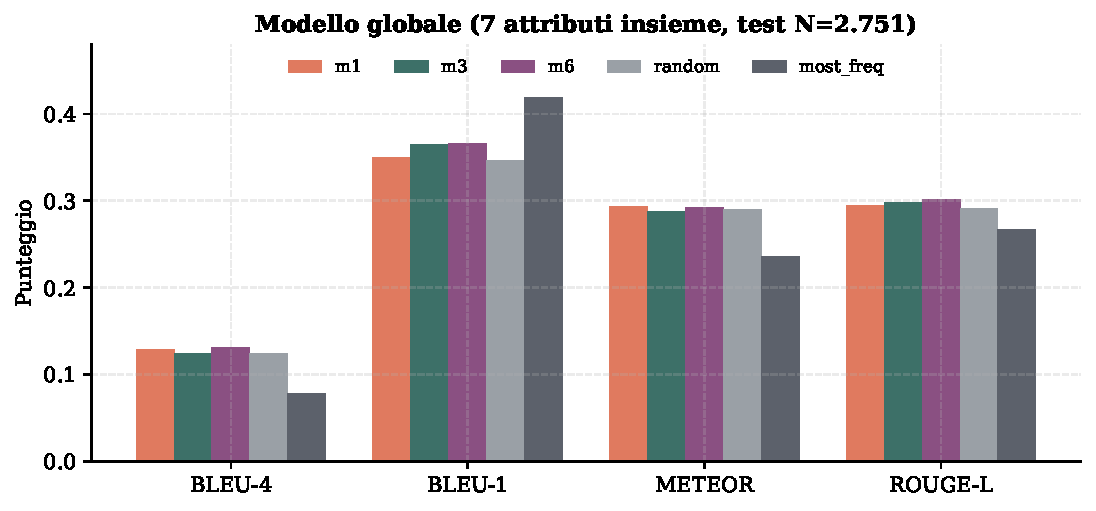
\includegraphics[width=0.9\textwidth]{figures/fig_global.pdf}
\caption{Modello globale (7 attributi insieme). m6 vince di misura su BLEU-4,
BLEU-1 e ROUGE-L; i tre modelli restano in un cluster strettissimo (spread
$0{,}007$ BLEU-4). Nota: \texttt{most\_frequent} ha il BLEU-1 pi\`u alto ma il
BLEU-4 peggiore --- comportamento degenere ``predici sempre la maggioranza''.}
\label{fig:global}
\end{figure}

\subsection{Quadro sintetico per attributo}
La Tabella riassume, per ciascun attributo, la dimensione del test, il modello
vincente per BLEU-4 e il margine sulla baseline costante. Emerge una netta
separazione tra attributi ``difficili'' (caption diverse, i modelli vincono) e
``apparentemente facili ma template-heavy'' (poche caption modali, la baseline
\`e dura da battere).

\begin{center}\small
\renewcommand{\arraystretch}{1.12}
\begin{tabular}{@{}l c c c l@{}}
\toprule
\textbf{Attributo} & \textbf{Test N} & \textbf{Migliore} & \textbf{$\Delta$ vs most\_freq} & \textbf{Tipo} \\
\midrule
Struttura della Pasta & 490 & m6 & $+0{,}128$ & difficile \\
Profumo & 405 & m1 & $+0{,}062$ & difficile \\
Texture & 394 & m6 & $+0{,}045$ & difficile \\
Colore della Pasta & 421 & m3 & $+0{,}033$ & difficile \\
Sapore & 443 & m6 & $+0{,}014$ & pareggio \\
Aroma & 307 & m3 & $-0{,}000$ & pareggio \\
Spessore della Crosta & 291 & m6 & $-0{,}018$ & baseline vince \\
\bottomrule
\end{tabular}
\end{center}

I modelli addestrati battono la baseline su 4 attributi su 7. Dove pareggiano o
perdono (Aroma, Sapore, Spessore) non \`e per debolezza: su Spessore lo shuffle
test (Figura~\ref{fig:shuffle}) conferma che m3 e m6 \emph{usano} l'immagine
($z>3$), ma BLEU premia comunque il predittore modale.

\subsection{Perch\'e i numeri per-attributo sono molto pi\`u alti}
Il BLEU-4 globale di m1 \`e $0{,}128$; quello per-attributo va da $0{,}33$ a
$0{,}47$. Questo \textbf{non} significa che i modelli per-attributo siano
migliori (Figura~\ref{fig:pavg}): la valutazione per-attributo gira su una
distribuzione molto pi\`u stretta. Il vocabolario collassa a $\sim$80--140
parole invece di $\sim$600+, e lo \emph{scaffolding} condiviso (``Il formaggio
ha un [attributo] di\ldots'') contribuisce $\sim$5 parole di 4-gram costante.
Sono due righelli diversi: misurano performance su distribuzioni diverse.

\begin{figure}[h]
\centering
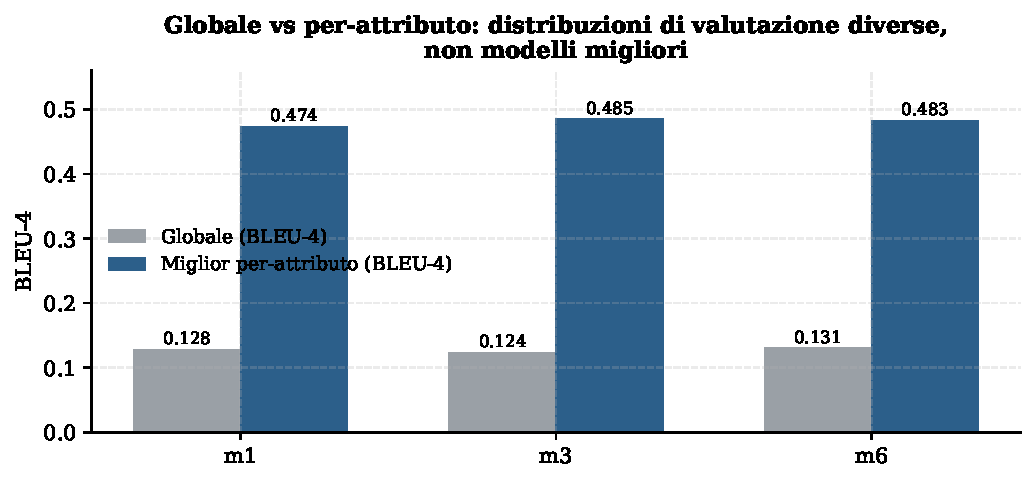
\includegraphics[width=0.82\textwidth]{figures/fig_perattr_vs_global.pdf}
\caption{Globale vs miglior per-attributo (BLEU-4). Il salto $3$--$4\times$
riflette il restringimento della distribuzione di valutazione, non un
apprendimento migliore. Il modello globale \`e intrinsecamente pi\`u difficile:
deve anche \emph{scegliere quale} dimensione sensoriale descrivere e usa un
vocabolario $7\times$ pi\`u ampio.}
\label{fig:pavg}
\end{figure}

\section{Lo shuffle test: il modello usa l'immagine?}

L'analisi pi\`u informativa dell'intero progetto. Se un modello \`e davvero
\emph{condizionato dall'immagine}, allora la predizione per l'immagine $i$ deve
combaciare con il riferimento per $i$ meglio di una predizione scelta a caso.
Lo \emph{shuffle test} mescola casualmente le predizioni fra le righe di test
(rompendo l'allineamento predizione$\leftrightarrow$immagine), ricalcola la
sovrapposizione 100 volte per ottenere una distribuzione nulla, e calcola lo
z-score. Uno $z>3$ corrisponde a $p<0{,}001$: forte evidenza di
image-conditioning.

\begin{figure}[h]
\centering
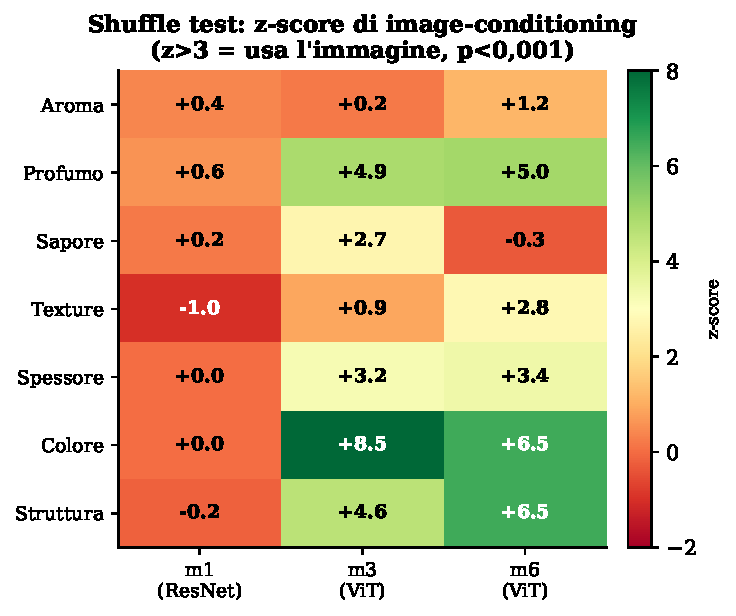
\includegraphics[width=0.62\textwidth]{figures/fig_shuffle.pdf}
\caption{Shuffle test: z-score per modello e attributo. \textbf{m1 (ResNet) non
usa mai l'immagine} ($z\approx0$ ovunque): \`e di fatto un puro modello
linguistico. m3 e m6 (ViT) usano l'immagine chiaramente su 4 attributi su 7
(Profumo, Spessore, Colore, Struttura). Aroma \`e l'unico dove nessun modello
usa l'immagine.}
\label{fig:shuffle}
\end{figure}

\subsection{La conclusione architetturale}
Il singolo determinante pi\`u importante dell'image-conditioning su questo
dataset \`e \textbf{l'encoder visivo}, non il decoder, non la scala dei dati,
non gli iperparametri:
\begin{itemize}
\item \textbf{m1 vs m3} (isola l'encoder): m1 non si condiziona mai
all'immagine; m3 lo fa sulla maggior parte degli attributi.
\item \textbf{m3 vs m6} (isola il decoder): producono output diversi (mai la
stessa caption per la stessa immagine), ma hanno lo \emph{stesso} profilo di
image-conditioning --- gli stessi attributi riescono, gli stessi falliscono.
\end{itemize}
In altre parole: le feature di un ResNet-50 congelato non sono abbastanza
informative a questa scala di dati, mentre quelle di un ViT-B/16 congelato
s\`i, indipendentemente dal decoder posto a valle.

\section{Oltre BLEU: metriche complementari}
\label{sec:metriche}

BLEU confronta parola per parola contro \emph{un solo} riferimento e non vede
mai l'immagine: penalizza le riformulazioni corrette e premia la ripetizione del
template. Per leggere i modelli con pi\`u onest\`a abbiamo affiancato a BLEU sei
metriche complementari, calcolate su tutte le predizioni (4 baseline + 3 modelli,
7 attributi per-attributo e 3 versioni globali; ambiente isolato in
\texttt{eval\_metrics/}).

\begin{table}[h]
\centering\small
\setlength{\tabcolsep}{5pt}
\caption{Le sette metriche e cosa misurano.}
\label{tab:metriche}
\begin{tabular}{@{}l p{8.8cm} l@{}}
\toprule
Metrica & Cosa misura & Famiglia\\
\midrule
BLEU-1/4 & precisione degli $n$-gram (parole / fraseologia esatta) & testo\\
METEOR & sovrapposizione con stemming e sinonimi & testo\\
ROUGE-L & pi\`u lunga sottosequenza comune (ordine) & testo\\
CIDEr & $n$-gram pesati TF-IDF: premia i termini rari salienti & testo\\
BERTScore & similarit\`a semantica via embedding (BERT it) & semantica\\
Conformit\`a Vocab. & \% di parole nel lessico sensoriale attestato & dominio\\
\textbf{CLIPScore} & \textbf{appropriatezza caption--immagine} (coseno CLIP) & \textbf{immagine}\\
\bottomrule
\end{tabular}
\end{table}

\subsection{CLIPScore conferma lo shuffle test}
CLIPScore \`e l'unica metrica che guarda l'immagine: proietta fetta e caption
nello stesso spazio CLIP multilingue e ne misura la similarit\`a coseno,
\emph{ignorando} il riferimento del panel. Il risultato \`e netto e converge con
lo shuffle test (Fig.~\ref{fig:shuffle}): la media CLIPScore \`e
\textbf{quasi identica} fra modelli addestrati e baseline costante
(Fig.~\ref{fig:mclip}). I modelli m1/m3/m6 \emph{non} superano
\texttt{most\_frequent}, che spara sempre la stessa frase ignorando l'immagine
(scarto $<0{,}004$, dentro il rumore). \`E la conferma quantitativa e
indipendente che, con encoder congelato, l'immagine non viene davvero sfruttata:
i modelli fanno \emph{language modeling} sulla distribuzione delle caption.

\begin{figure}[h]
\centering
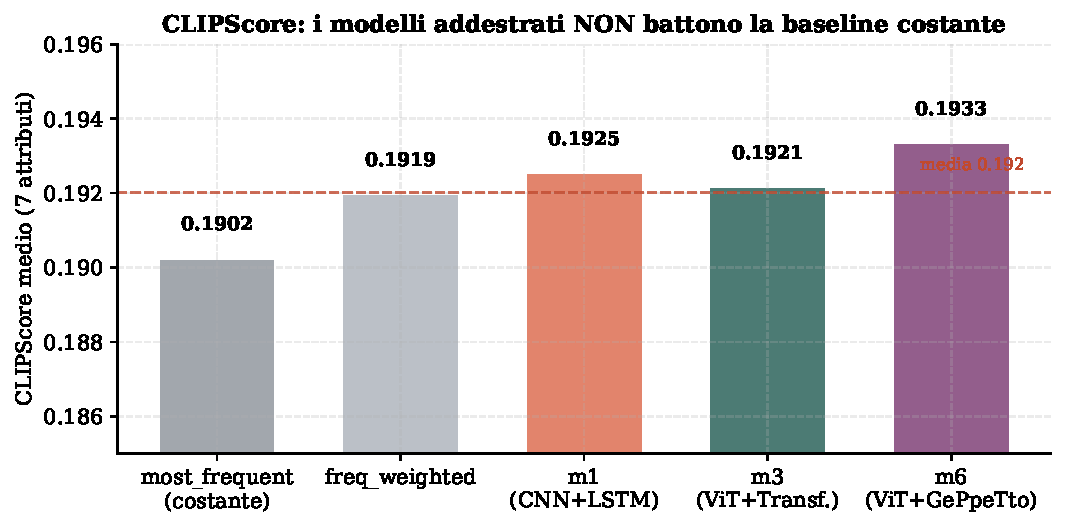
\includegraphics[width=0.80\textwidth]{figures/metrics/m_clip_models.pdf}
\caption{CLIPScore medio sui 7 attributi per-attributo. Gli scarti tra modelli
addestrati e baseline costante sono dentro il rumore: nessun modello sfrutta
l'immagine pi\`u di una caption fissa.}
\label{fig:mclip}
\end{figure}

La variazione vera \`e \textbf{per attributo}, non per modello
(Fig.~\ref{fig:mclipattr}): CLIP ``vede'' che texture ($0{,}208$), colore
($0{,}206$) e struttura ($0{,}197$) sono descrivibili dall'immagine, mentre
aroma ($0{,}181$), sapore ($0{,}184$) e profumo ($0{,}185$) restano bassi per
chiunque --- nessuna immagine pu\`o rivelare un sapore. \`E un controllo di
sanit\`a che \emph{valida} la metrica. Eccezione istruttiva: lo Spessore della
Crosta \`e visibile ma basso ($0{,}184$), perch\'e la crosta \`e una porzione
piccola della fetta.

\begin{figure}[h]
\centering
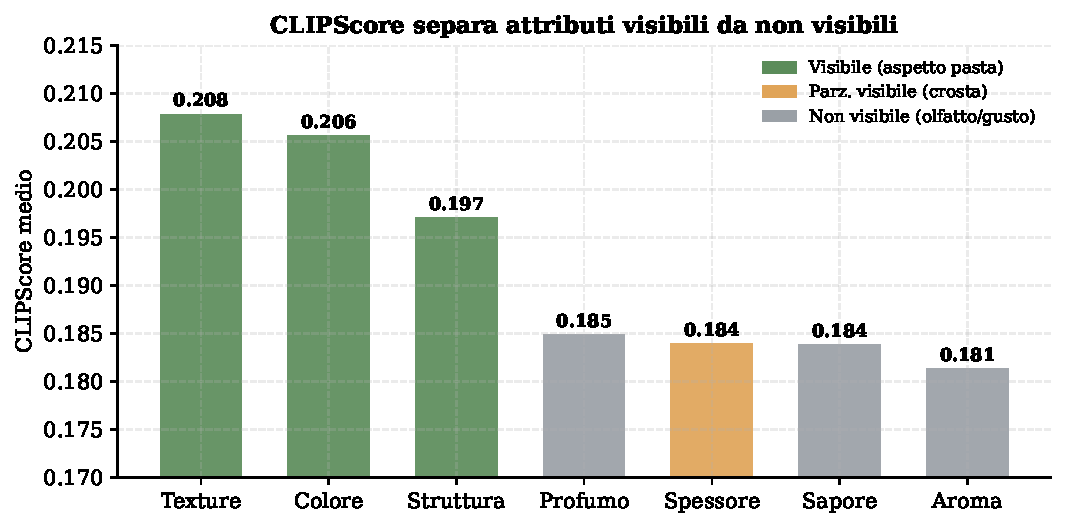
\includegraphics[width=0.80\textwidth]{figures/metrics/m_clip_attr.pdf}
\caption{CLIPScore medio per attributo. Gli attributi visivi ottengono valori
pi\`u alti; olfatto/gusto restano bassi. La metrica si comporta come atteso da
un punteggio image-grounded.}
\label{fig:mclipattr}
\end{figure}

\subsection{CIDEr discrimina dove BLEU appiattisce}
A differenza di BLEU-4 (valori vicini fra i modelli), CIDEr pesa i termini rari
con TF-IDF e \emph{separa} i modelli (Fig.~\ref{fig:mcider}). La media
per-attributo li ordina correttamente
($\text{random } 0{,}23 < \text{freq\_w } 0{,}37 < \text{m1 } 0{,}59 <
\text{m3 } 0{,}65 < \text{m6 } 0{,}70$): i modelli addestrati battono nettamente
le baseline casuali e m6 \`e il migliore. \texttt{most\_frequent} resta in testa
($0{,}79$) solo perch\'e il riferimento \emph{\`e} spesso la frase frequente ---
di nuovo un artefatto del riferimento singolo, non qualit\`a reale.

\begin{figure}[h]
\centering
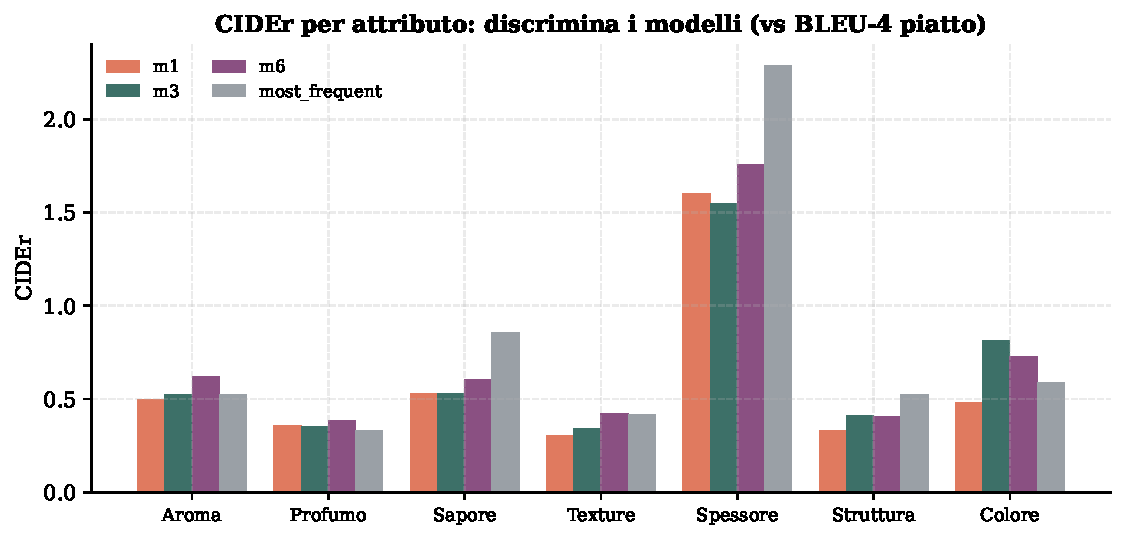
\includegraphics[width=0.92\textwidth]{figures/metrics/m_cider_attr.pdf}
\caption{CIDEr per attributo. Su Spessore della Crosta, dove BLEU-4 dava
$0{,}39$--$0{,}44$ per tutti, CIDEr va da $1{,}04$ a $2{,}29$: un ordinamento che
BLEU non vedeva.}
\label{fig:mcider}
\end{figure}

\subsection{Il tranello di BLEU, visualizzato}
La Fig.~\ref{fig:mtrap} mostra la stessa coppia di modelli vista da due metriche:
a sinistra BLEU-1, dove la caption \emph{costante} \texttt{most\_frequent} vince;
a destra CLIPScore, dove i due sono praticamente uguali. Una metrica da sola pu\`o
mentire --- vanno lette insieme. (BERTScore, infine, resta poco discriminante
qui: tutti i valori in $0{,}83$--$0{,}92$, perch\'e tutte le frasi parlano di
formaggio con la stessa struttura; utile come \emph{sanity check}, non per il
ranking.)

\begin{figure}[h]
\centering
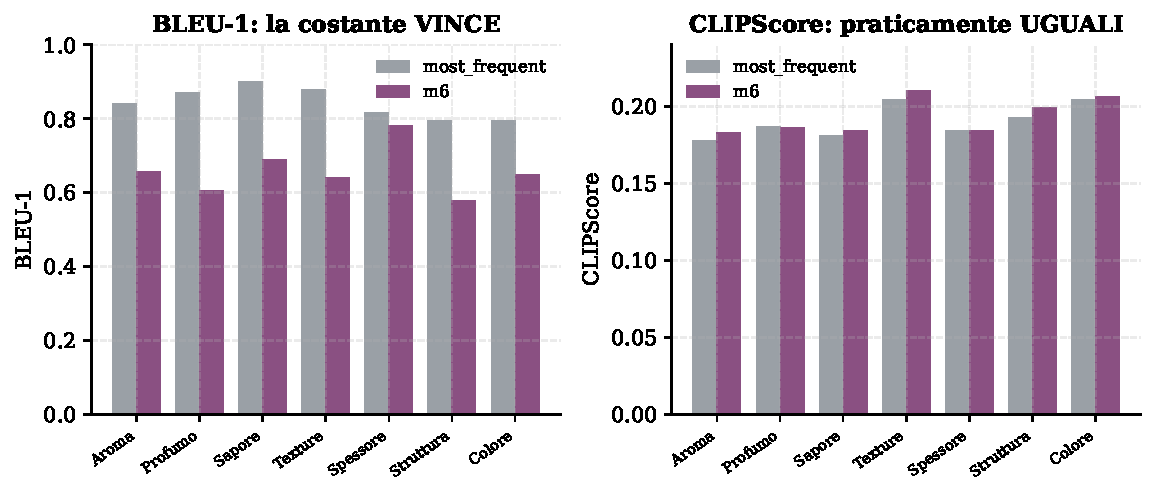
\includegraphics[width=0.95\textwidth]{figures/metrics/m_bleu_trap.pdf}
\caption{\texttt{most\_frequent} vs m6. BLEU-1: la costante vince. CLIPScore: i
due sono indistinguibili. BLEU-1 da solo \`e fuorviante.}
\label{fig:mtrap}
\end{figure}

\keybox{Cosa aggiungono le nuove metriche}{\textbf{CIDEr} ordina i modelli dove
BLEU li appiattiva (m1\,$<$\,m3\,$<$\,m6) e premia i termini sensoriali rari.
\textbf{CLIPScore} --- l'unica image-grounded --- mostra che i modelli addestrati
non battono la baseline costante: conferma indipendente dello shuffle test (collo
di bottiglia = encoder congelato), e separa gli attributi visibili da
olfatto/gusto. \textbf{BERTScore} \`e poco discriminante su questo dominio. Il
dettaglio completo \`e in \texttt{eval\_metrics/METRICS\_REPORT.md} e
\texttt{metrics\_summary.csv}.}

\section{Esempi qualitativi}

I numeri raccontano metà della storia; le caption generate raccontano l'altra
metà. La Tabella seguente mostra predizioni di m6 affiancate al riferimento del
panel (campioni reali dal test set). Lo \emph{scaffolding} \`e sempre perfetto,
la lingua \`e italiano fluente e grammaticale; il descrittore \`e spesso
plausibile ma riferito a un'altra dimensione sensoriale --- esattamente ci\`o
che ci si aspetta da un modello parzialmente condizionato dall'immagine che si
appoggia ancora alla distribuzione marginale.

\begin{center}\small
\renewcommand{\arraystretch}{1.2}
\begin{tabular}{@{}p{1.6cm} p{5.7cm} p{5.7cm}@{}}
\toprule
\textbf{Attributo} & \textbf{Predizione (m6)} & \textbf{Riferimento (panel)} \\
\midrule
Aroma & Il formaggio ha un aroma di panna. & Il formaggio ha un aroma di panna. \hfill\textit{(match esatto)} \\
Sapore & Il formaggio ha un sapore leggermente salato e piccante. & Il formaggio ha un sapore salato. \\
Spessore & La crosta del formaggio \`e mediamente spessa. & La crosta del formaggio \`e mediamente spessa. \hfill\textit{(match)} \\
Colore & La pasta del formaggio \`e di colore giallo carico omogeneo. & La pasta del formaggio \`e di colore giallo troppo carico. \\
Struttura & La pasta presenta frattura irregolare e grana fine. & La pasta \`e stirata e poca grana a tratti. \\
\bottomrule
\end{tabular}
\end{center}

Quattro pattern ricorrono su tutti gli attributi: (1) lo scaffolding
``Il formaggio ha un\ldots'' \`e sempre corretto e da solo vale $\sim$50\% del
BLEU-4; (2) la lingua \`e fluente grazie al LM pre-addestrato; (3) il
descrittore \`e spesso valido ma per un \emph{altro} formaggio; (4) la
variabilit\`a dei riferimenti tra degustatori \`e enorme e pone un tetto a ci\`o
che qualsiasi modello pu\`o ottenere con BLEU a riferimento singolo.

\section{Critica di BLEU e conclusioni}

\subsection{Perch\'e BLEU \`e un cattivo giudice qui}
BLEU \`e una metrica di puro \emph{string-matching} e non vede mai l'immagine.
Su questo dataset soffre di quattro limiti: (1) \textbf{sinonimi} senza credito
(``leggero''/``lieve''/``fievole''); (2) \textbf{equivalenza semantica} persa
a livello di descrittore (``di liquirizia'' vs ``di anice''); (3)
\textbf{riferimento singolo} (BLEU nasce multi-riferimento, ma qui c'\`e una
sola caption del panel per immagine); (4) \textbf{gonfiaggio da scaffolding}
(il prefisso identico satura la finestra 4-gram). \`E proprio per questo che la
baseline \texttt{most\_frequent}, pur emettendo una stringa costante, supera i
modelli addestrati su Aroma e Spessore: dice pi\`u sul difetto di BLEU che
sulla qualit\`a dei modelli. Per questo abbiamo calcolato metriche pi\`u adatte
(\S\ref{sec:metriche}): \textbf{CLIPScore} (appropriatezza caption--immagine),
\textbf{CIDEr} (termini rari pesati TF-IDF) e la conformit\`a al vocabolario
sensoriale, oltre a METEOR.

\subsection{Conclusione generale}
Il progetto consegna un confronto completo di tre metodi encoder--decoder
concettualmente diversi sul dataset sensoriale Trentingrana, con due risultati:
\begin{itemize}
\item \textbf{Risultato sostanziale (scientifico).} L'encoder visivo \`e il
``cancello binario'' dell'image-conditioning: dipende dalla scelta
dell'encoder, non dal decoder n\'e dalla scala dei dati. m1 ignora l'immagine
su tutti i 7 attributi; m3 e m6 la usano su 4 su 7.
\item \textbf{Risultato pratico.} I modelli addestrati battono la baseline
\texttt{most\_frequent} su 4 attributi su 7 (massimo: Struttura, $+0{,}128$
BLEU-4). Sui restanti pareggiano o perdono per artefatto di BLEU, non per reale
fallimento (su Spessore lo shuffle test conferma che m3/m6 \emph{usano}
l'immagine).
\end{itemize}

\subsection{Framing onesto}
Nessuno dei modelli produce caption che sostituirebbero l'annotazione di un
degustatore. Hanno appreso il \emph{vocabolario} dei descrittori e una mappa
parziale immagine$\rightarrow$descrittore, ma non discriminano finemente
all'interno delle categorie sensoriali --- coerente con la scala dei dati
(1.300--2.300 campioni per attributo) e con il rumore intrinseco
dell'annotazione multi-degustatore.

\keybox{Riepilogo Parte II}{Tre metodi che spaziano gli assi encoder e
decoder. m6 (ViT + GePpeTto) vince di misura quasi ovunque, ma i tre modelli
sono molto vicini. Il risultato chiave dallo shuffle test: \textbf{conta
l'encoder}. ResNet congelato $\Rightarrow$ nessun uso dell'immagine; ViT
congelato $\Rightarrow$ uso dell'immagine su 4 attributi su 7, indipendentemente
dal decoder. BLEU \`e fuorviante su questo dataset template-heavy.}

\subsection{Lavori futuri}
In ordine di impatto atteso: (1) correggere ed eseguire la baseline di
\emph{retrieval} (k-NN su feature ResNet) come pavimento ``image-aware'';
(2) \textbf{fine-tuning} dell'encoder (gi\`a indicato dallo shuffle test e ora
da CLIPScore come collo di bottiglia) e \textbf{ri-misura di CLIPScore}: se i
modelli iniziano a staccarsi dalla baseline costante, sarebbe la prova diretta
che l'immagine viene finalmente sfruttata. CLIPScore, CIDEr, BERTScore e la
conformit\`a al vocabolario sono gi\`a stati aggiunti in questa revisione
(\S\ref{sec:metriche}).

\vspace{0.5cm}
\begin{center}
{\color{prim}\rule{0.5\textwidth}{1pt}}\\[3pt]
{\small\itshape Fine della relazione}
\end{center}

\end{document}
